 \documentclass[11pt]{article}

%_______packages___________________________________________________

%package for including figures 

\usepackage{graphicx}

%packages from the American Mathematical Society - good for symbols and various constructions
\usepackage{titlesec}
\usepackage{amsmath}
\usepackage{amssymb}

%package to include colour (color) in the text - can be convenient to highlight material, particularly when working on draft material

\usepackage{color}

\usepackage{xcolor}


%package for listing code, here Matlab 

\usepackage{listings}

\usepackage{multicol}
\setlength{\columnsep}{1cm}
\title{Second multicols Demo}

%_______commands to make the best use of space on a page________________

\parindent=0pt
\parskip=8.0pt
\baselineskip=12pt
\oddsidemargin=-0.5cm
\textwidth=17cm
\topmargin=-1.4cm
\textheight=23.0cm

%_______settings for listing computer code using the listings package________________

\definecolor{codegreen}{rgb}{0,0.6,0}
\definecolor{codegray}{rgb}{0.5,0.5,0.5}
\definecolor{codepurple}{rgb}{0.58,0,0.82}
\definecolor{backcolour}{rgb}{0.95,0.95,0.92}
\lstdefinestyle{mystyle}{
    backgroundcolor=\color{backcolour},   
    commentstyle=\color{codegreen},
    keywordstyle=\color{magenta},
    numberstyle=\tiny\color{codegray},
    stringstyle=\color{codepurple},
    basicstyle=\ttfamily\footnotesize,
    breakatwhitespace=false,         
    breaklines=true,                 
    captionpos=b,                    
    keepspaces=true,                 
    numbers=none,                    
    numbersep=5pt,                  
    showspaces=false,                
    showstringspaces=false,
    showtabs=false,                  
    tabsize=2}
\lstset{style=mystyle}

\usepackage{float}
\usepackage{tabularx}

%_______end of preamble and start the document proper________________


\begin{document}

{\large\bf MTH2005 Modelling: Theory and Practice }
 
\vspace{4mm} 

{\Large\bf Numerical Solutions in Financial Mathematics - The Black-Scholes Equation - Dr Ben Snow }

\vspace{1mm}

Group 1: Elliot Lawrence (710046334), Tom Bailey-Burnley (710041568), Sofia Fernandez-Hearn (720005519), Bertie Tufnell (70003485), Daisy Macharg (720052934), Jeremy Brown (710045257)

\vspace{3mm}

\section{Week 1 Tasks} % To be removed when tasks below are completed

\section{Introduction}

The Black-Scholes equation is a fundamental finance equation which can be derived from the roots of mathematical principles, it serves as a key use in understanding the complexities of pricing dynamics of options. This report focuses on numerically solving the Black-Scholes equation, aiming to understand how option values change with varying current prices (£5, £15, £20). 

In addition to deriving the Black-Scholes equation, we look deeper to its relationship to the diffusion equation, understanding what core mathematical ideas are used.  Using finite difference methods like Crank-Nicolson and Successive Over-Relaxation, we also navigate the Black-Scholes equation backwards in time from the final condition \(C(S, T)\).

At the end of this report, we also aim to assess the accuracy and stability of our solutions we have calculated and give examples showing the impact of how various scenarios can influence option prices.



\section{What is the Black-Scholes Equation}

Before introducing the Black-Scholes Equation, lets first define what a call option is. A call option is when you have the right but not the obligation to, purchase a stock at a pre-agreed upon price at a later date. The pre-agreed upon price is known as the strike price.

There are different types of call options for example: A European call option, is were you are only allowed to exercise the option on a particular date. This is different from the American call option, for which you can purchase the stock any time upto a particular date.\ In both cases we call this particular date, the expiry date. 

Let's consider an example of a European call option: Let's say you buy an option to purchase a stock at \textsterling $£100$ on the the $25^{th}$March for \textsterling $10$. In Figure 1, we can see in practice how exercising this option might be done.
If the price of the stock rises above \textsterling$10$ to let's say to \textsterling$130$.\ We could then buy the stock at \textsterling$100$ and sell it for \textsterling$20$ profit. Alternatively if the price of the stock falls below the strike price, we can chose not to buy the stock and just lose \textsterling$10$.
\begin{figure}[H]
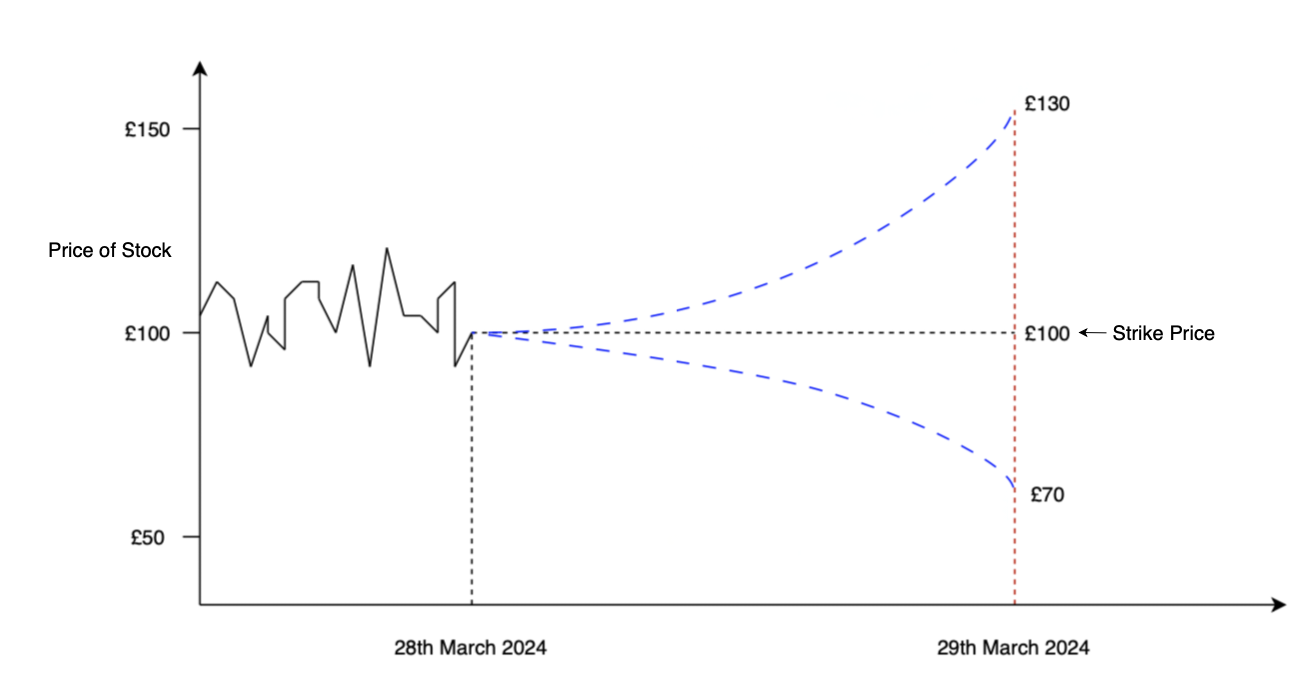
\includegraphics[width=1\linewidth, height=9cm]{Call-option.png}
\caption{An example of a European Call option}
\end{figure}
As we can see the process of exercising a call option is a straight forward process. The real challenge is in, how to decided on the price to sell them at. This issue has baffled people ever since call options were invented, and that's why we have the Black-Scholes equation.

The Black-Scholes equation is a mathematical model used in finance to calculate the theoretical price of European call options.

The equation was developed by economists Fischer Black and Myron Scholes in 1973.

The Black-Scholes equation for a European call option is given by:

\[ \frac{\partial C}{\partial t} + \frac{\sigma^2S^2}{2} \frac{\partial^2 C}{\partial S^2} + rS \frac{\partial C}{\partial S} - rC = 0 \]

Where:
\begin{itemize}
    \item \(C(S, t)\) represents the price of a financial option.
    \item \(\frac{\partial C}{\partial t}\) represents how the option price changes overtime.
    \item \(\frac{\partial C}{\partial S}\) represents how the option price changes with respect to stock price.
    \item \(S\) represents the current stock price.
    \item \(\sigma\) represents the volatility of the stock.
    \item \(r\) represents the risk-free interest rate.
\end{itemize}

\newpage


\section{Derivation of the Black-Scholes Equation}

Before we derive the Black-Scholes Equation, we must introduce the idea of Ito processes.
Ito processes are a type of stochastic process ,i.e they are a set of random variables describing the evolution of system over time.\ Ito process are stochastic processes which exhibit the Markov property.\ In the context of financial mathematics, the Markov property states that the future value of a financial stock option is independent of the past values it has taken. An example of an Ito process is,
\begin{equation*}
dX = a(X,t)dz + b(X,t)dt 
\end{equation*}
Where the functions $a(X,t)dz$ and $b(X,t)dt$, are called the diffusion and drift terms respectively. The value of a stock price varies randomly over time, so we can model how it changes using a Ito process. To derive the Black-Scholes Equation we must assume that the current stock price can be modelled by a particular Ito process, known as Geometric Brownian motion. With this type of Ito process there is only one random variable. We make this assumption so that the probability density of S must have a log-normal distribution.\ This ensures, that the price of stock cannot take negatives values.

Shown in equation (1), is the stock price following a Geometric Brownian motion:
\begin{equation}
dS = \sigma S dX + \mu S dt 
\end{equation}
In equation (1), the drift term contains $\mu $.\ This represents the average growth rate of the stock price. The diffusion term, $\sigma S dX$ is a stochastic process were $dX$ is a random variable and $\sigma$ is the volatility of the stock. The volatility of a stock, are the random fluctuations of the price around the average growth rate.\ For deriving the Black-Scholes Equation we assume that it is a known constant. Note that, the drift and diffusion terms are proportional to S. This property distinguishes Geometric Brownian motion from the arithmetic case.

Now before we continue with the derivation, we must introduce an crucial lemma.

\subsection{Ito's Lemmma}
Ito's lemma was invented by a Japanese mathematician in the late $20^{th}$century.\
The lemma relates infinitesimal changes of a function containing a random variable to infinitesimal changes in the random variable itself. In other words, it acts as the chain rule in a stochastic setting.

Assume x follows an Ito process given by the following:
\begin{equation*}
dX = a(X,t)dz + b(X,t)dt 
\end{equation*}
This is similar to the example of a Ito process from before, but we will assume $dz$ is a Wiener process and the variable $X$ has a variance rate of $b^2$. A Wiener process is another example of an Ito process, but the drift and diffusion terms are not functions of t.

Ito's lemma states that a function of the variable x, for example $f(t,X(x,t))$ can be expressed as,
\begin{equation*}
df = \frac{\delta f}{\delta X}adz + 
\setlength{\arraycolsep}{2pt}\begin{pmatrix} \frac{\delta f}{\delta X}b + \frac{\delta f}{\delta t} + \frac{1}{2}\frac{\delta^2 f}{\delta X^2}a^2\end{pmatrix}dt\phantom{cccc}
\end{equation*}
This is equivalent to a Taylor series expansion of $df$, followed by an application of the multiplication identities and the lemma applied to $dz^2$.\ The Taylor series expansion (2) and multiplication identities are shown below.
\begin{equation}
df = \frac{\delta f}{\delta t}dt + \frac{\delta f}{\delta z}dz + \frac{1}{2}\frac{\delta^2 f}{\delta z^2}dz^2
+\frac{1}{2}\frac{\delta^2 f}{\delta t^2}dt^2 + \frac{\delta^2 f}{\delta S \delta t}dtdz + ...
\end{equation}

\begin{center}
\begin{tabular}{  c|  c  c}
x & $dt$ & $dz$ \\
\hline
$dt$ & 0 & 0  \\ 
$dz$ & 0 & $dt$  \\ 
\end{tabular}
\end{center}

To derive the Black-Scholes equation we will apply Ito's lemma to the price of a financial option, $C(t,S)$ in a similar way. First, Let's apply Ito's lemma to $dS^2$. This will be useful later when dealing with $dC(t,S)$
\begin{equation*}
dS^2 = (\sigma S dX + \mu S dt)^2
\end{equation*}
\vspace{-10pt}
\begin{equation*}
\phantom{ccccccccccccccccccccccc}
= \sigma ^2 S^2 dX^2 + 2\mu \sigma S^2 dXdt + \mu ^2 S^2 dX^2
\end{equation*}
Applying, the multiplication identities allows u to simplify the equation. Note, that for this situation our $dz$ stated in Ito's lemma is $dX$.
\vspace{-5pt}
\begin{equation*}
\phantom{cccccccccccccccccc}
= \sigma ^2 S^2 dt + \mu ^2 S^2 dt\phantom{cccccccccccccc}
\end{equation*}
 The leading term $\sigma ^2 S^2 dX^2$, gives us the smallest power of dt. If we take $dt <1$ and consider $dt$ as it tends to zero, then this leading term dominates the equation. Thus we can approximate $dS^2 \approx \sigma ^2 S^2 dt$.


The price of a financial option,
expressed as a Taylor expansion is shown in equation (3).
\\
\begin{equation}
dC = \frac{\delta C}{\delta t}dt + \frac{\delta C}{\delta S}dS + \frac{1}{2}\frac{\delta^2 C}{\delta S^2}dS^2
+\frac{1}{2}\frac{\delta^2 C}{\delta t^2}dt^2 + \frac{\delta^2 C}{\delta S \delta t}dtdS
\end{equation}

In equation (4) we've left out the first term of the expansion, $C(0,0)$ as it's value is just zero. We can then apply the multiplication identity $dt^2 = 0$ from Ito's lemma and simplify the equation to,
\begin{equation}
dC = \frac{\delta C}{\delta t}dt + \frac{\delta C}{\delta S}dS + \frac{1}{2}\frac{\delta^2 C}{\delta S^2}dS^2
+ \frac{\delta^2 C}{\delta S \delta t}dtdS
\end{equation}
Substituting our expressions for $dS$ and $dS^2$ gives us equation(5) as follows:
\begin{equation}
dC =\frac{\delta C}{\delta t}dt + \frac{\delta C}{\delta S}(\sigma S dX + \mu S dt) + \frac{1}{2}\frac{\delta^2 C}{\delta S^2}(\sigma ^2 S^2 dt^2)+ \frac{\delta^2 C}{\delta S \delta t}(\sigma S dXdt + \mu S dt^2)
\end{equation}
\begin{equation*}
dC = \frac{\delta C}{\delta t}dt + \frac{\delta C}{\delta S}(\sigma S dX + \mu S dt) + \frac{1}{2}\frac{\delta^2 C}{\delta S^2}(\sigma ^2 S^2 dt^2)
\end{equation*}
\begin{equation*}
dC = \sigma S \frac{\delta C}{\delta S}dX + 
\setlength{\arraycolsep}{2pt}\begin{pmatrix} \mu S \frac{\delta C}{\delta S} + \frac{1}{2}\sigma^2 S^2\frac{\delta^2 C}{\delta S^2} + \frac{\delta C}{\delta t}\end{pmatrix}dt\phantom{cccc}
\end{equation*}

Now let's construct a portfolio, consisting entirely of one stock option $C(t,S)$,
\begin{equation}
\pi = C(t,S) - \Delta S
\end{equation}
Here $\Delta$S scales the underlying option and in doing so adjusts the values of the option $\pi$. We will see later what an optimal choice for $\Delta$ might be.
From the equation above we can calculate an expression for the return on the portfolio,
\begin{equation}
d\pi = dC(t,S) - \Delta dS
\end{equation}
Now let's substitute in our expressions for $dC$ and $dS$ into the equation:
\begin{equation*}
d \pi = \sigma S \frac{\delta C}{\delta S}dX + 
\setlength{\arraycolsep}{2pt}\begin{pmatrix} \mu S \frac{\delta C}{\delta S} + \frac{1}{2}\sigma^2 S^2\frac{\delta^2 C}{\delta S^2} + \frac{\delta C}{\delta t}\end{pmatrix}dt - \Delta(\sigma S dX + \mu S dt)
\end{equation*}
\begin{equation*}
= \sigma S \setlength{\arraycolsep}{2pt}\begin{pmatrix} \frac{\delta C}{\delta S} - \Delta \end{pmatrix}dX + 
\setlength{\arraycolsep}{2pt}\begin{pmatrix} \mu S \frac{\delta C}{\delta S} + \frac{1}{2}\sigma^2 S^2\frac{\delta^2 C}{\delta S^2} + \frac{\delta C}{\delta t} - \Delta S \mu
\end{pmatrix}dt \phantom{ccc}
\end{equation*}
Now it's clear to see that an optimal choice for $\Delta$ would be, $\Delta = \frac{\delta C}{\delta S}$ as this would eliminate the random component of the SDE. The equation then becomes,
\begin{equation*}
d \pi = 
\setlength{\arraycolsep}{2pt}\begin{pmatrix}
\frac{\delta C}{\delta t} + \frac{1}{2}\sigma^2 S^2\frac{\delta^2 C}{\delta S^2}
\end{pmatrix}dt \phantom{ccc}
\end{equation*}
For deriving the Black-Scholes Equation, we must assume there is no Arbitrage. Arbitrage is the process of buying and selling the same stock in different markets to profit from very small difference in the stock price. When we assume there is no Arbitrage we are assuming that the portfolio will grow at a risk free rate, also known as the rate of inflation. As a result we can let $d \pi = r\pi dt$ were $r$ is the risk free rate, which we have assumed over a short period time. From this the Black-Scholes Equation follows:
\begin{equation*}
\pi dt = 
\setlength{\arraycolsep}{2pt}\begin{pmatrix}
\frac{\delta C}{\delta t} + \frac{1}{2}\sigma^2 S^2\frac{\delta^2 C}{\delta S^2}
\end{pmatrix}dt \phantom{ccc}
\end{equation*}
\begin{equation*}
r(C-\Delta S)dt = 
\setlength{\arraycolsep}{2pt}\begin{pmatrix}
\frac{\delta C}{\delta t} + \frac{1}{2}\sigma^2 S^2\frac{\delta^2 C}{\delta S^2}
\end{pmatrix}dt \phantom{ccc}
\end{equation*}
Equivalently we can say that,
\begin{equation*}
\frac{\delta C}{\delta t} + \frac{1}{2}\sigma^2 S^2 \frac{\delta ^2 C}{\delta S^2} + rS \frac{\delta C}{\delta S} - rC = 0
\end{equation*}

\section{How the Black-Scholes Equation relates to the Diffusion Equation}

\subsection{Elliot's Draft}

The Black-Scholes equation is a partial differential equation (PDE) that describes the evolution of the option price over time. Its form is similar to the diffusion equation. We can use the descriptions below to see the relationship.


The diffusion equation, a fundamental mathematical model, describes the spread of a quantity in space over time. Its basic form is expressed as:
\[ \frac{\partial u}{\partial t} = D \frac{\partial^2 u}{\partial x^2} \]
Here, \(u\) signifies the quantity being diffused (e.g., heat), \(t\) denotes time, \(x\) represents space, and \(D\) is the diffusion coefficient. This equation captures how the quantity dynamically propagates through space over time. Analogously, the diffusion process can be likened to the spread of heat in a room, with the diffusion coefficient (\(D\)) determining the rate of heat permeation.


In financial mathematics, the Black-Scholes equation serves as a diffusion model for option prices, expressed as:
\[ \frac{\partial C}{\partial t} + \frac{\sigma^2S^2}{2} \frac{\partial^2 C}{\partial S^2} + rS \frac{\partial C}{\partial S} - rC = 0 \]

The middle term:

\[\frac{\sigma^2S^2}{2} \frac{\partial^2 C}{\partial S^2} \]

Can be seen as the diffusion term in Black-Scholes

Here, \(C\) represents the option price, \(S\) is the current stock price and \(\sigma\) reflects the stock's volatility This equation encapsulates the influences of stock price changes, volatility, and interest rates on option prices over time. Similarly to the diffusion of heat, envisioning the option price (\(C\)) as a dynamic quantity, the stock price (\(S\)) as a spatial variable and the volatility (\(\sigma\)) as the unpredictability in option price movement, . The Black-Scholes equation offers a predictive framework for how option prices evolve over time in response to how it relates to

\newpage


\subsection{Sofia's Draft}
The Black-Scholes equation describes the price of a call option as time goes on, it can be transformed into the diffusion equation when we take into account its boundary conditions and some of the assumptions made to construct the model. Remember that the Black-Scholes equation is the following:
\[\frac{\partial C}{\partial t} + \sigma^2 S^2 \frac{\partial^2 C}{\partial S^2} + rS \frac{\partial C}{\partial S} - rC = 0
\]
Wherein C is the price of the call option, S is the price of the underlying stock, and t is time. r is the risk-free interest rate and $\sigma $ is the volatility of the stock.

For the boundary conditions regarding the value of the underlying stock, we have $C(0,t)=0$ and $C(S,t)\approx S$ as $S \rightarrow \infty$. Additionally, if the day at maturity of the option is T then $C(S,T)=max(S-k,0)$, for an exercise price of $k$. This final condition means that we will be working backwards in time from $T$, as we have a condition for the final price of the option and we want to find its price earlier in time. Let us also define two functions, $\Tilde{S}$ and $\Tilde{C}$ which will appropriately represent the change in the direction of time. For these two new expressions, $S_t = \Tilde{S}_\tau$ and $C_t = \Tilde{C}_\tau$
This gives us the first variable transformation.
\[
\tau = T - t
\] Wherein $\tau$ represents the time remaining until the maturity of the option.

Using just this variable change, and being careful with notation, we get that
\begin{align*}
    \frac{\partial C}{\partial S} &= \frac{\partial \Tilde{C}}{\partial \Tilde{S}} \\
    \frac{\partial C}{\partial t} &= -\frac{\partial \Tilde{C}}{\partial \tau}
\end{align*}

We can then substitute these into the original PDE to have an expression that moves forwards in $\tau$ (ie. backwards in time.) This will give us
\[
- \frac{\partial \Tilde{C}}{\partial \tau} + \frac{\sigma^2 \Tilde{S}^2}{2} \frac{\partial^2 \Tilde{C}}{\partial \Tilde{S}^2} + r \Tilde{S} \frac{\partial \Tilde{C}}{\partial \Tilde{S}} - r \Tilde{C} = 0
\]

As the price of the stock is assumed to follow Brownian motion, the value of the stock, ignoring the stochastic term (why?) at the exercise date $T$ is given by
\[
S_T = e^{\ln{S_T}+(r-\frac{1}{2}\sigma^2)(T-\tau) }
\]

find logarithm, explain variables

\[
x = \ln{\Tilde{S}_\tau} + (r-\frac{1}{2} \sigma^2)\tau
\]

forward value of option 
\[
F_\tau = C_\tau e^{r\tau}
\]

differentiating (twice wrt S)
explain notation
\[
\frac{\partial \Tilde{C}}{\partial \Tilde{S}} = \frac{1}{\Tilde{S}}\frac{\partial c}{\partial x}
\]
\[
\frac{\partial^2 \Tilde{C}}{\partial \Tilde{S}^2} = \frac{1}{\Tilde{S}} \left( -\frac{\partial c}{\partial x} + \frac{\partial^2 c}{\partial x^2}\right)
\]

also have the total derivative wrt tau
\[
\frac{\partial \Tilde{C}}{\partial \tau} = \frac{\partial c}{\partial \tau} + \frac{\partial c}{\partial x}\left( r - \frac{1}{2}\sigma^2 \right)
\]

We can then substitute these derivatives into the partial derivative (going forwards in time) that we previously found. This gives us the following expression:

\[
\frac{\partial c}{\partial \tau} + \frac{1}{2} \sigma^2 \frac{\partial^2 c}{\partial x^2} - rc = 0
\]

We can then find the derivatives wrt tau and x of the function we proposed for the future value of the option, to plug them into that equation.
have
\[
c = Fe^{r \tau}
\]

\[
\frac{\partial c}{\partial x} = e^{-r \tau} \frac{\partial F}{\partial x}
\]
\[
\frac{\partial^2 c}{\partial x^2} = e^{-r \tau} \frac{\partial^2 F}{\partial x^2}
\]
\[
\frac{\partial c}{\partial \tau} = e^{-r \tau}\frac{\partial F}{\partial \tau} - r F e^{-r \tau}
\]


Substituting this into the previous pde (which is in terms of partial dervatives of c) we will get 
\[
-\left( e^{-r \tau}\frac{\partial F}{\partial \tau} - r F e^{-r \tau} \right) + \frac{1}{2}\sigma^2 e^{-r \tau} \frac{\partial^2 F}{\partial x^2} - r F e^{-r \tau} = 0
\]

When simplified and terms moved to appropriate side this expression is 
\[
\frac{1}{2} \sigma^2 \frac{\partial^2 F}{\partial x^2} = \frac{\partial F}{\partial \tau}
\] 
Which is the diffusion equation with constant $\frac{\sigma^2}{2}$. 

This equation would have boundary conditions \[
F(x,0) = max(e^{\frac{1}{2}(a+1)x }- e^{\frac{1}{2}(a-1)x} , 0)
    \] for $a = \frac{2r}{\sigma^2}$



\subsection{Sofia's Draft (for pde without diffusion constant)}

An alternative way of converting the Black-Scholes PDE is through using the mathematical properties of the model to adapt it into a diffusion equation without drift. We start with the following variable transformations.
\[ S = Ke^x \hspace{1.5cm} \tau = \frac{\sigma^2}{2}(T-t) \hspace{1.5cm} C(s,t) = K f(x,\tau)\]

We can then differentiate C in respect to time and using the product rule, find an expression for $\frac{\partial C}{\partial t}$ in terms of $f$, $\tau$ and other cosntants.

\begin{align*}
    \frac{\partial C}{\partial t} &= K\frac{\partial f}{\partial \tau} \frac{\partial \tau}{\partial t} \\
     &= -\frac{K \sigma^2}{2} \frac{\partial f}{\partial \tau}
\end{align*}

We then differentiate $C$ with respect to $S$ twice, to get the necessary expressions.


\begin{align*}
    \frac{\partial C}{\partial S} & = K \left( \frac{\partial f}{\partial x} \frac{\partial x}{\partial S} \right) \\
    &= \frac{K}{S} \frac{\partial f}{\partial x} 
\end{align*}

\begin{align*}
    \frac{\partial^2 C}{\partial S^2} &= K \frac{\partial}{\partial S} \left( \frac{1}{S} \frac{\partial f}{\partial x} \right) \\
    & extra working? \\
    &= \frac{K}{S^2} \left( \frac{\partial^2}{\partial x^2} - \frac{\partial f}{\partial x} \right)
\end{align*}

We can then substitute these expressions into the original PDE. This will remove the terms $S$ and $S^2$ multiplying the first and second derivatives of $C$ and also make it an equation going forward in $\tau$ rather than backwards in $t$.

\[-\frac{K\sigma^2}{2} \frac{\partial f}{\partial \tau} + \frac{\sigma^2 S^2}{2} \left(\frac{K}{S^2}\left(\frac{\partial^2 f}{\partial x^2} -\frac{\partial f}{\partial x} \right) \right) + rS\frac{K}{S}\frac{\partial f}{\partial x} - rKf = 0\]

\[
-\frac{\partial f}{\partial \tau} + \frac{ \partial^2 f}{\partial x^2} - \frac{\partial f}{\partial x} + \frac{\sigma^2 r}{2}\frac{\partial f}{\partial x} -\frac{\sigma^2 r}{2} f = 0
\]

\hspace{5cm}Letting $c = \frac{\sigma^2 r}{2}$
\[
\frac{\partial f}{\partial \tau} + \frac{ \partial^2 f}{\partial x^2} + (c-1) \frac{\partial f}{\partial x} - cf = 0
\] At this point, the intital condition has changed to $f(x, 0) = max(e^x -1 , 0)$

This has transformed the Black-Scholes PDE into a diffusion equation with drift, so we can use another transformation of variables to turn it into a diffusion equation without drift. we choose \[f (x, \tau) = e^{ax+b\tau} f(x,\tau)\]  and then find appropriate $a$ and $b$ terms so that the new diffusion equation has no drift.

We have the following derivatives of $f$:

\begin{align*}
    \frac{\partial f}{\partial \tau} &= be^{ax+b\tau} u + \frac{\partial u}{\partial \tau} e^{ax+b\tau} \\
    &= \left(bu+\frac{\partial u}{\partial \tau} \right) e^{ax+b\tau}
\end{align*}
\begin{align*}
    \frac{\partial f}{\partial x} = \left(au + \frac{\partial u}{\partial x} \right) e^{ax+b\tau}
\end{align*}

\begin{align*}
    \frac{\partial^2 f}{\partial x^2} = \left( \frac{\partial^2 u}{\partial x^2} + 2a\frac{\partial u}{\partial x} + a^2 \right) e^{ax+b\tau}
\end{align*}

We can the substitute these expressions into our forward PDE:

\[
-\left(bu + \frac{\partial u}{\partial \tau} \right)e^{ax+b\tau} + \left(\frac{\partial^2 f}{\partial x^2} = \left( \frac{\partial^2 u}{\partial x^2} + 2a\frac{\partial u}{\partial x} + a^2 \right) \right) e^{ax+b\tau} + (c-1)\left (au + \frac{\partial u}{\partial x} \right) e^{ax+b\tau} - cue^{ax+b\tau} = 0
\]

To ensure that we have no drift terms, we want the coefficients of $u$ and $\frac{\partial u}{\partial x}$ to be equal to zero. we get this by choosing
\[
a = -\frac{1}{2}(c-1)  \;\; \text{and}  \;\; b = -\frac{1} {4}(c+1)^2
\]

We will then have the diffusion equation (without drift)

\[
\frac{\partial u}{\partial \tau} = \frac{\partial^2 u}{\partial x^2} \;\; \text{for} \;\; -\infty < x < \infty \;\; \text{and} \;\; \tau >0
\]

Adapting the initial condition (again) we will also have 
\[
u(x,0) = max(e^{\frac{1}{2}(c+1)x}- e^{\frac{1}{2}(c-1)x} , 0 )
\]

\newpage
\section{Week 2 Tasks} % To be removed when tasks below are completed

\section{Crank-Nicholson Scheme} 

\subsection{Elliot's Draft}


\subsection{Crank-Nicholson Derivation}

The Crank-Nicholson scheme stands out as a robust and stable numerical method compared to both the implicit and explicit methods. This is because small mistakes won't be as impactful in later computations as seen in the implicit and explicit methods. Although this method requires extra computational work and time, it serves as a reliable choice in financial applications where precision takes precedence over speed and where the consequences of errors can be profound.

The graphical representation below offers a reason why it makes sense the explicit and implicit methods are called what they are. The explicit method uses information at the given time to help predict a future value, and the implicit method uses a value in the future to predict the current value. The Crank Nicholson method uses an amalgamation of these methods. It blends the characteristics of the explicit and implicit methods, providing a balanced numerical method that inherits the strengths of both methodologies.

\begin{figure}[H]
    \centering
    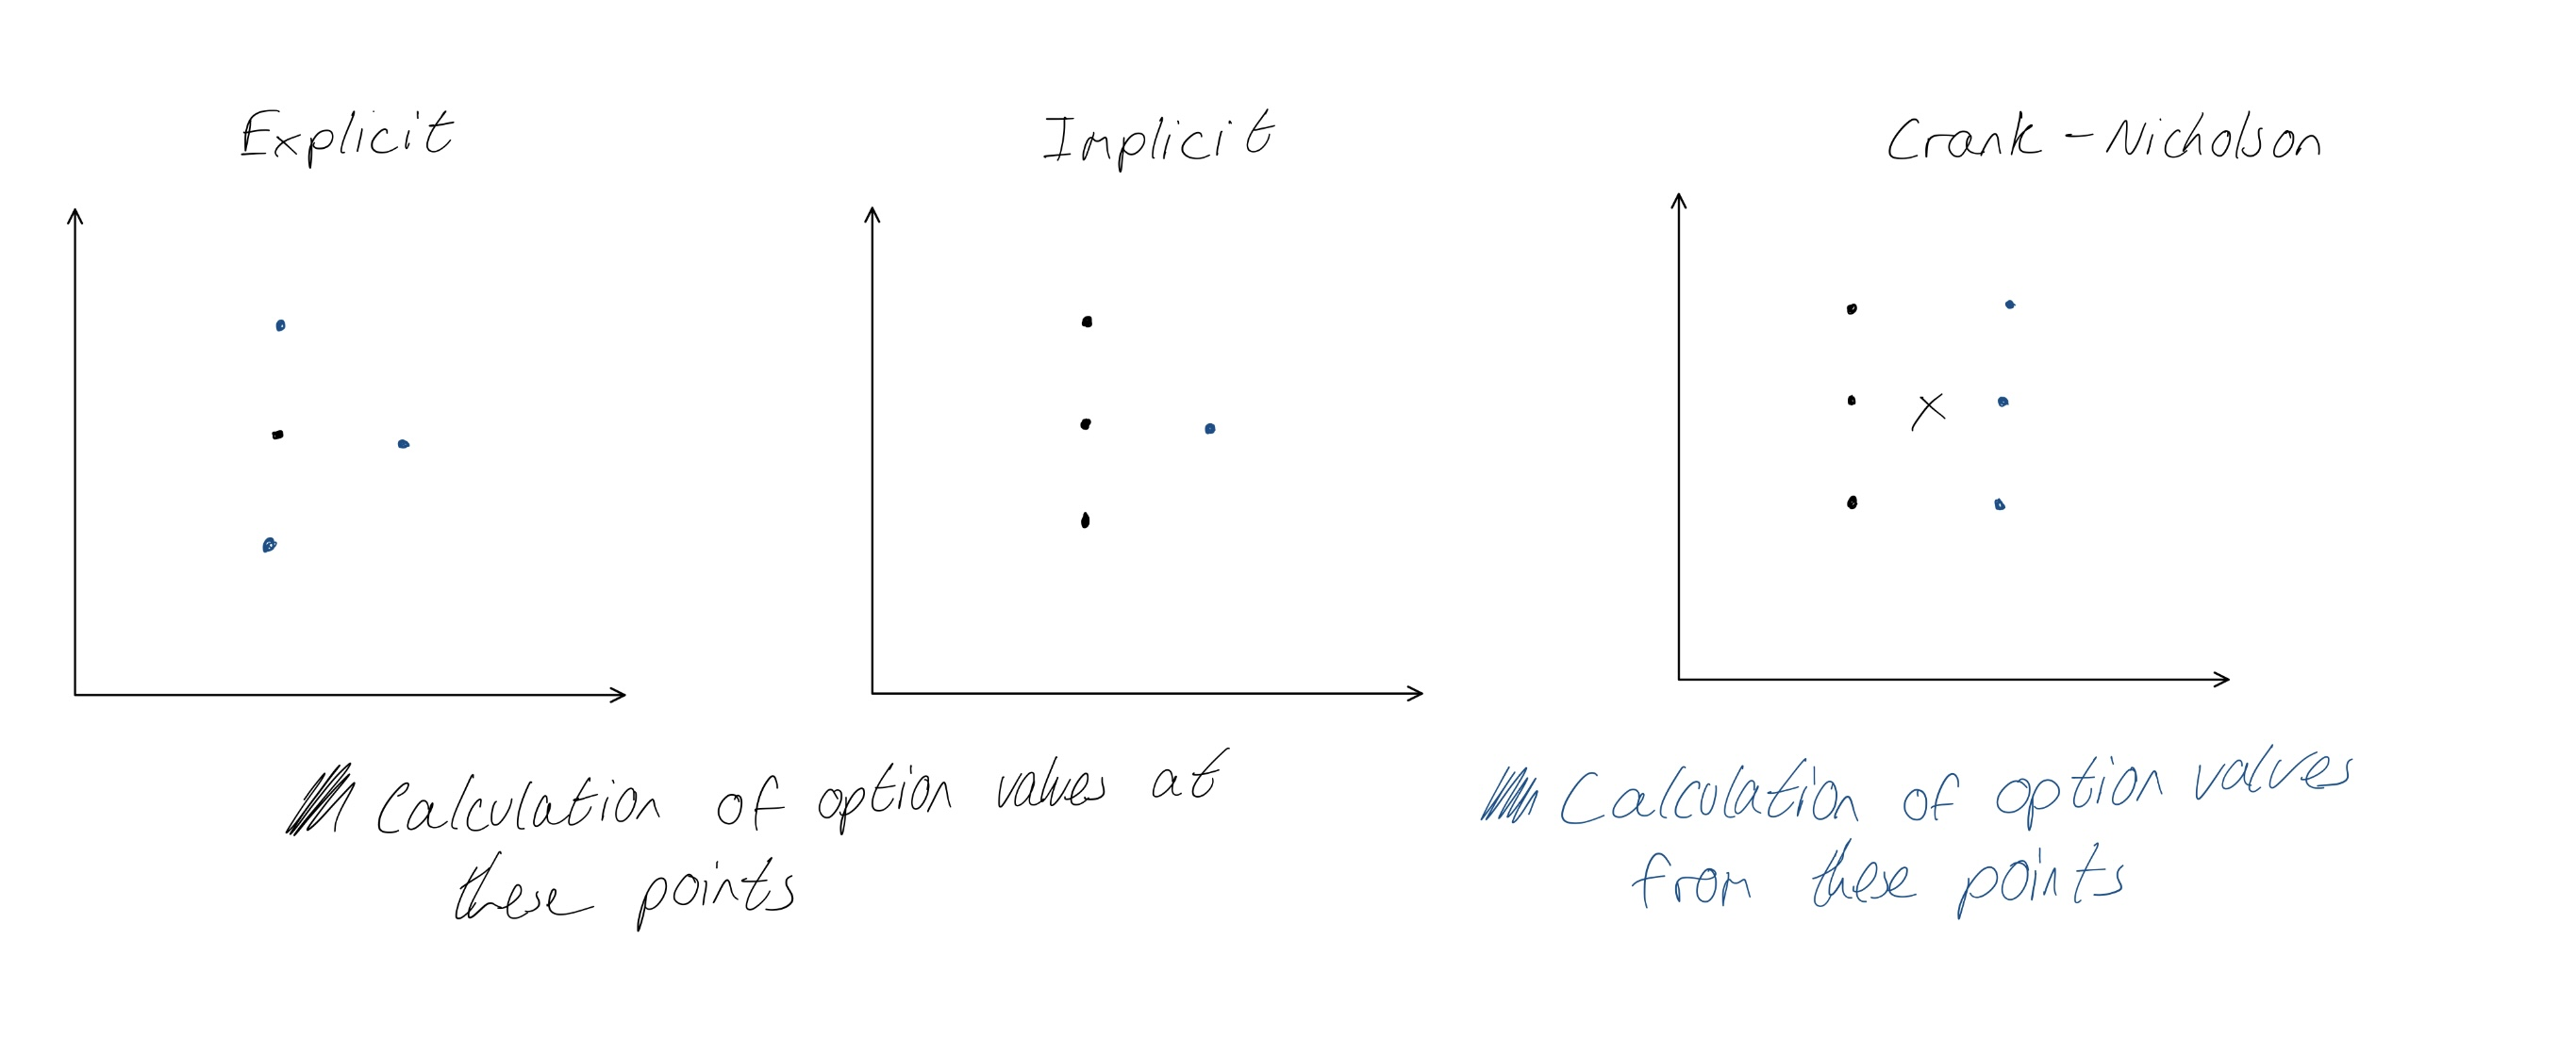
\includegraphics[width=1\linewidth]{Crank-Nicholson-GR.jpg}
    \caption{Comparison of the explicit, implicit and Crank-Nicholson methods}
    \label{}
\end{figure}

More specifically, from the explicit method, it borrows the idea of:

\begin{itemize}

\item Using the current time step values to estimate future values. This aspect contributes to the method's intuitiveness and easy implementation
\end{itemize}
From the implicit method, it incorporates the idea of:
\begin{itemize}
\item The stability and accuracy, especially for smaller steps, by considering future time step values in its calculations
\end{itemize}

The Crank-Nicholson method can be represented as a differential equation

\[
\frac{{(V_i)^{n+1} - (V_i)^n}}{{\Delta t}} = \frac{1}{2} \left( f(V^n) + f(V^{n+1}) \right)
\]

The left side represents the option values at the next and current time steps respectfully, and f(V) represents the function defining the change in option value. The right side of the equation is an average of the function f(V) evaluated at the current and next time steps. This goes back to the idea that the Crank-Nicholson idea uses the "average" of both the explicit and implicit methods. The \( f(V^n) \) and \( f(V^{n+1}) \) are implicit and explicit methods, respectfully.







\section{Berties CN draft}

BS $\to$ Diffusion equation: $\frac{\partial u}{\partial \tau}=\frac{\partial^2u}{\partial x^2}$\\
$u$ represents option value
$\tau$ represents transformed time variable
$x$ represents transformed spatial variable

\begin{align*}
    \frac{u_i^{j+1}-u+i^j}{\Delta \tau}=\frac{1}{2}\left(\frac{u_{i+1}^{j+1}-2u_i^{j+1}+u_{i-1}^{j+1}}{\Delta x^2}+\frac{u_{i+1}^{j}-2u_i^{j}+u_{i-1}^{j}}{\Delta x^2}\right)
\end{align*}

Now let $r=\frac{\Delta\tau}{2\Delta x^2}$ (constant), and collect $j+1$ terms on the left and $j$ terms on the right:

\begin{align*}
    -ru_{i-1}^{j+1}+(1+2r)u_i^{j+1}-ru_{i+1}^{j+1}=ru_{i-1}^j+(1-2r)u_i^j+ru_{i+1}^j
\end{align*}

This can be converted to a matrix equation $\mathbf{Au^{j+1}=Bu^j}$:

\begin{align*}
    &\left(\begin{array}{ccccccc}
        X & & & & & &\\
        & \ddots & & & & &\\
        & -r & 1+2r & -r & & &\\
        & & -r & 1+2r & -r & &\\
        & & & -r & 1+2r & -r &\\
        & & & & & \ddots &\\
        & & & & & & X
    \end{array}\right)\left(\begin{array}{c}
        \vdots \\
        u_{i-1}^{j+1}\\
        u_{i}^{j+1}\\
        u_{i+1}^{j+1}\\
        \vdots
    \end{array}\right)\\
    =&
    \left(\begin{array}{ccccccc}
        X & & & & & &  \\
        & \ddots & & & & & \\
        & r & 1-2r & r & & &\\
        & & r & 1-2r & r & &\\
        & & & r & 1-2r & r & \\
        & & & & & \ddots &\\
        & & & & & & X
    \end{array}\right)\left(\begin{array}{c}
        \vdots \\
        u_{i-1}^{j}\\
        u_{i}^{j}\\
        u_{i+1}^{j}\\
        \vdots
    \end{array}\right)
\end{align*}

\subsubsection{MATLAB Code}

To Be Coded

\subsection{Successive over Relaxation}

\newpage

\subsubsection{Daisy's Draft}
In numerical linear algebra, the method of Successive Over-Relaxation (SOR) is a variant of the Gauss-Seidel method for solving a linear system of equations, resulting in faster convergence. Devised simultaneously by David M. Young Jr. and by Stanley P. Frankel in 1950 for the purpose of automatically solving linear systems on digital computers; it has become one of the most important methods for the solution of large linear systems. 
Given a square system of n linear equations with unknown x : Ax=b where  
\begin{figure}[H]
    \centering
    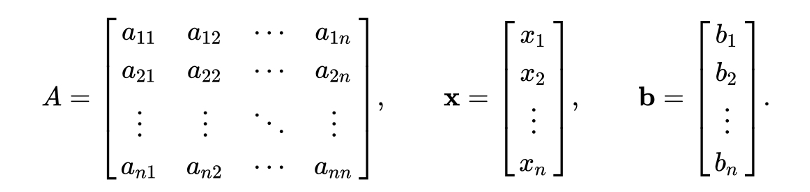
\includegraphics[width=0.5\linewidth]{image.png}
    \caption{Enter Caption}
    \label{fig:enter-label}
\end{figure}

we use the method of successive over-relaxation which is an iterative technique to solve for x. To do this we can decompose A as A = D + L + U  where
D is the diagonal part, L the lower triangular part, U the upper triangular part. Where The system of linear equations may be rewritten as:

\begin{figure}[H]
    \centering
    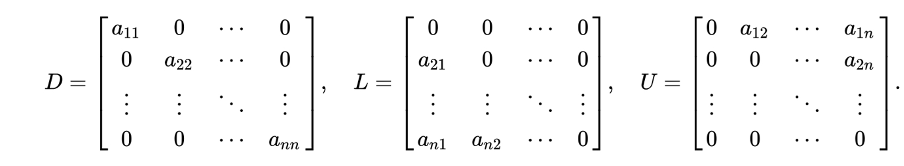
\includegraphics[width=0.5\linewidth]{image2.png}
    \caption{Enter Caption}
    \label{fig:enter-label}
\end{figure}

$(D+L)x = b- Ux$

Now to obtain the Gauss-Seidel scheme we make it iterative

$X^{k+1} = (D+L)^{-1}(b-Ux^K)$

Now the SOR variation of  Gauss-Seidel is achieved by implementing a relaxation parameter/factor into the scheme and setting 

$X_0^{k+1}=(D+L)^{-1}(b-Ux^K)$

$X^{k+1} = \omega x_0^k+1+x^k(1-\omega)$

Poor choice of the relaxation parameter $\omega$ can lead to poor convergence rates. On the other hand, a good choice of $\omega$ can lead to very fast convergence compared to the Jacobi or Gauss-Seidel methods. The spectral radius of BSOR is the eigenvalue of BSOR with maximum magnitude, and we want to choose $\omega$ so that $|\rho(BSOR (\omega))|$ is a minimum. Finding the optimal value of $\omega$ is very difficult in general, and the optimal value is known only for special types of matrices.
We use $w>1$ to put the greatest weight on the newly computed values. If $\vert BSOR \vert>1$ for some subordinate norm or $\rho(BSOR)<1$, the SOR iteration converges. 

Over-Relaxation methods were used before the work of Young and Frankel however these previous methods were designed for computation by human calculators which required some expertise to ensure convergence to the solution meaning they were inapplicable for programming on digital computers. An example of this would be the work of Lewis Fry Richardson, and the methods developed by R.V. Southwell. The SOR method has applications in many areas such as computational fluid dynamics, mathematical programming, medical analysis, and machine learning etc.
There is a Projected  Successive Over-Relaxation (PSOR) variation which is obtained by taking the relevant maximum of equation ***** with the option payoff function. These methods work provided the matrix is diagonally dominant and $0 < w < 2$.  Projected Successive Over-Relaxation (PSOR) can be notably enhanced by considering the intrinsic physical characteristics of the specific problem at hand. This improvement can be demonstrated in scenarios involving LCPs related to Moving Boundary Problems and the Valuation of American Options. These types of problems often necessitate a time-stepping approach, wherein a series of discrete LCPs must be solved, each corresponding to a specific time step. Within such contexts, there exists a dynamic boundary separating distinct domains with varying solution properties. By separating the problem into distinct boundaries, PSOR can be effectively applied to tasks with lower dimensions. This leads to a newly developed iterative approach that speeds up the process by up to 50\% when compared to traditional PSOR methods.

While Successive-Over Relaxation (SOR) is computationally demanding for solving linear equations, it needs less storage than Gauss-Seidel, making it more efficient. As data size and problem complexity increase, serial computing struggles to keep up. Parallelizing computationally intensive tasks like SOR becomes vital. Recent advancements in data generation and problem complexity highlight the importance and relevance of SOR in solving complex problems.

The Successive Over-Relaxation (SOR) method is now widely used in numerical linear algebra. It can solve large linear systems faster than other methods. It uses a relaxation parameter to make it more efficient. SOR can be applied to many fields, such as computational fluid dynamics, mathematical programming, and machine learning. An improved version of SOR, called Projected SOR (PSOR), is even more efficient for problems with moving boundaries or options valuation. SOR's efficiency and its ability to be used in parallel make it well-suited to address the growing computational demands in scientific research.

\section{Week 3 Tasks} % To be removed when tasks below are completed

\subsection{Von Neumann stability analysis}

\subsection{Complete SOR}

\subsection{Complete CN}
\section{References}



\end{document}